\documentclass[tikz,10pt]{standalone}

%%%%%%%%%%%%%%%%%%%%%%%%%%%%%%%%%%%%%%%%%
%                                       %
%                MY COLORS              %
%                                       %
%%%%%%%%%%%%%%%%%%%%%%%%%%%%%%%%%%%%%%%%%
 \definecolor{ccred}{cmyk}{0, 0.87, 0.8, 0.21}
 \definecolor{ccgreen}{RGB}{147,187,42}
 \definecolor{ccargile}{RGB}{239,239,239}
 %%%%%%%%%%%%%%%%%%%%%%%%%%%%%%%%%%%%%%%%%

\begin{document}
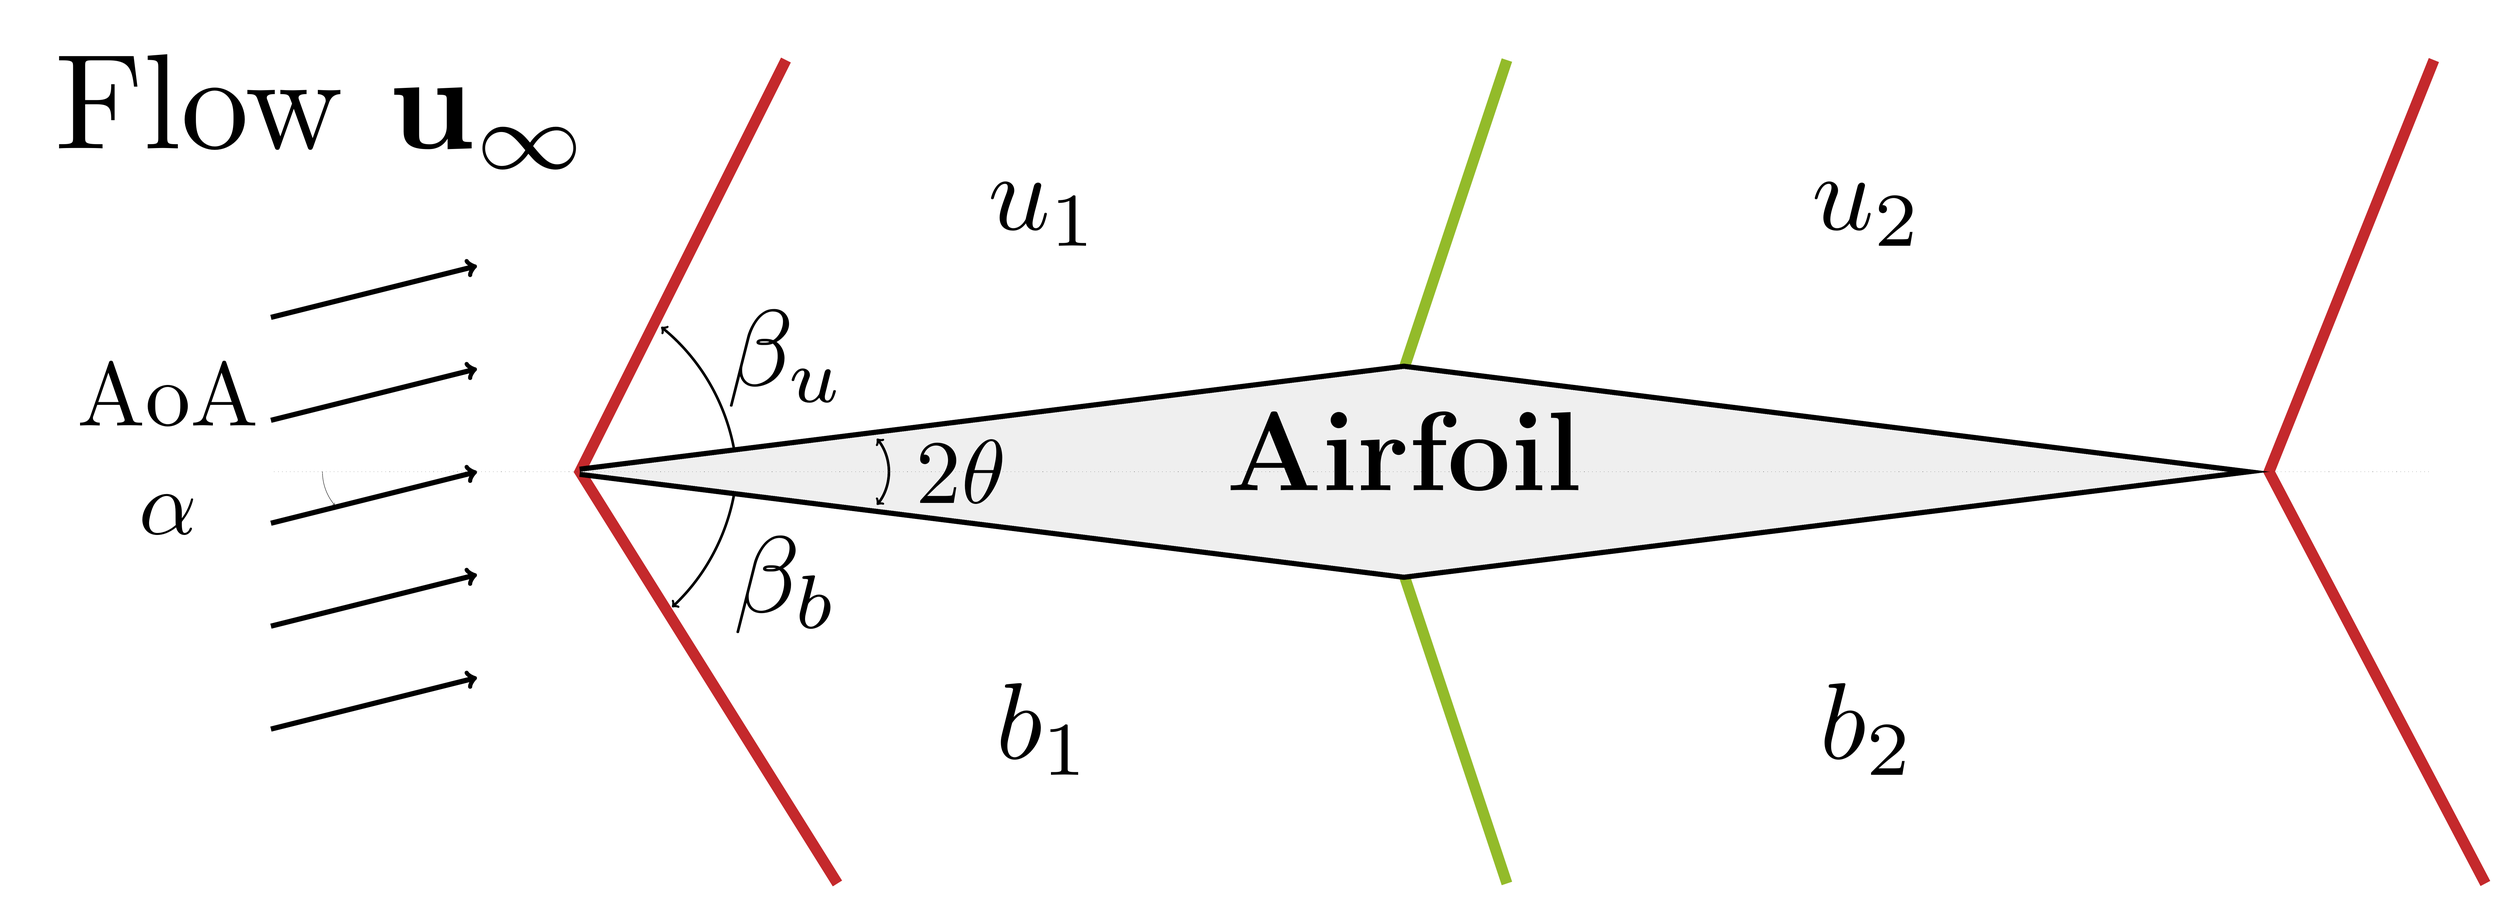
\begin{tikzpicture}[scale=4]

  % Choc
  \draw[line width=4.25mm, ccred] (0.5,-4) -- (-2,0) -- (0,4);
  \draw[line width=4.25mm, ccred] (16.5,-4) -- (14.4,0) -- (16,4);

  % Upper zone 1
  \draw[->, line width=1mm] (-0.5,0.2) arc (10:51:2cm);
  \draw(0,1.1) node[scale=12, black] (betau) {$\beta_{u}$};
  \draw(2.5,2.5) node[scale=12, black] (betau) {$u_1$};
  \draw(10.5,2.5) node[scale=12, black] (betau) {$u_2$};

  % Bottom zone 1
  \draw[->, line width=1mm] (-0.5,-0.2) arc (-10:-47:2cm);
  \draw(0,-1.1) node[scale=12, black] (betad) {$\beta_{b}$};
  \draw(2.5,-2.5) node[scale=12, black] (betau) {$b_1$};
  \draw(10.5,-2.5) node[scale=12, black] (betau) {$b_2$};
  
  % Détente
  \draw[line width=4.25mm, ccgreen] (6,1) -- (7,4);
  \draw[line width=4.25mm, ccgreen] (6,-1) -- (7,-4);
  
  % Vehicle
  \draw[line width=4mm] (-2,0) -- (6,1) -- (14,0) -- (6,-1) -- (-2,0) ;
  \draw[dotted, fill=ccargile] (-2,0) -- (6,1) -- (14,0) -- (6,-1) -- (-2,0) ;
  \draw[->, line width=1mm] (1,0) arc (0:40:0.5cm);
  \draw[->, line width=1mm] (1,0) arc (0:-40:0.5cm);
  \draw(1.7,0) node[scale=10, black] (beta) {2$\theta$};
  \draw(6,0.2) node[scale=5] (airfoil) {\Huge \textbf{Airfoil}};
  
  % Amont
  \draw[->, line width=2mm] (-5,-2.5) -- (-3,-2);
  \draw[->, line width=2mm] (-5,-1.5) -- (-3,-1);
  \draw[->, line width=2mm] (-5,-0.5) -- (-3,0);
  \draw[->, line width=2mm] (-5,0.5) -- (-3,1);
  \draw[->, line width=2mm] (-5,1.5) -- (-3,2);
  \draw(-4.5,3.5) node[scale=15, black] (ecoulement) { Flow $\mathbf{u_\infty}$};

  % Axis
  \draw (-5,0) node (begin) {};
  \draw (16,0) node (end) {};
  \draw[loosely dotted] (begin) -- (end) ;

  % AoA (Angle of Attack)
  \draw (-5,-0.5) node (u1) {};
  \draw (-3, 0) node (u2) {};
  \draw[->] (-4.5,0) arc (180:220:0.5cm);
  \draw(-6,0.8) node[scale=10, black, text width=1cm] (AoA) {\begin{center} AoA $\alpha$ \end{center}};
 

\end{tikzpicture}
\end{document}
